\newcommand\auteur{Tony Clavien, Maxime Guillod, Gabriel Luthier \& Guillaume Milani}
\newcommand\cours{GEN}
\newcommand\ecole{IL --- TIC --- HEIG-VD}
\newcommand\domaine{Mini-Projet}
\newcommand\titre{Frogger}
\newcommand\objectif{\item[\textit{Objectif :}]}
\newcommand\duree{\item[\textit{Dur\'ee :}]}
\newcommand\dateRendu{\item[\textit{Date du rendu :}]}
\newcommand\partageTache{\item[\textit{Partage des t\^aches :}]}
\newcommand\effort{\item[\textit{Effort :}]}

\documentclass[a4paper,12pt]{article}
%
\author{\auteur}
\title{\titre}
\date{\today}

\usepackage[frenchb]{babel}
\usepackage{fancyhdr}
\usepackage{graphicx}
\usepackage{amsmath}
\usepackage{listingsutf8}
\usepackage{color}
\usepackage{enumerate}
\usepackage[utf8]{inputenc}
\usepackage[T1]{fontenc}
\usepackage{float}
\usepackage{geometry}
\usepackage{amssymb,mathtools,pifont}
\usepackage{enumitem}
\usepackage{xspace}
\usepackage{appendix}
% Liens
\usepackage[hyphens]{url}
\usepackage{hyperref}
\geometry{verbose,tmargin=2.5cm,bmargin=2cm,lmargin=1.8cm,rmargin=1.8cm}
\selectlanguage{frenchb}
\frenchbsetup{StandardLists=true}
\DeclareGraphicsExtensions{.pdf,.png,.jpg}
\setlength\parindent{0pt}
\setlength{\parskip}{0.7em}

\usepackage{listings}
\lstset{
	breaklines=true, 
	basicstyle=\scriptsize,
	inputencoding=utf8/latin1,
	extendedchars=true,
	numbers=left,   
	firstnumber=1,
	numberfirstline=true, 
	language=Java,
	keywordstyle=\color{blue}\ttfamily,
	stringstyle=\color{red}\ttfamily,
	commentstyle=\color{black}\ttfamily
}


% headers & footers
\pagestyle{fancy}

\lhead{\domaine}
\rhead{\titre\space
\includegraphics[scale=0.03]{../Logo/logo.jpg}}

\renewcommand{\footrulewidth}{0.4pt}% default is 0pt
\lfoot{\auteur}
\cfoot{}
\rfoot{\thepage}

%%%%%%%%%%%%%%%%%%%%%%%%%%%%%%%%%%%%%%%
%%%%%%% BEGIN DOCUMENT
%%%%%%%%%%%%%%%%%%%%%%%%%%%%%%%%%%%%%%%

\begin{document}
	\clearpage\maketitle
	\thispagestyle{empty}
	
	\maketitle
	\begin{figure}[h!]
		\centering
		
\includegraphics[scale=0.7]{../Logo/logo.jpg}
	\end{figure}
	\newpage
	
	% % Entete première page
	% \thispagestyle{empty}
	% %
	% \noindent \cours \hfill \ecole{} \newline
	% \noindent \auteur \hfill \today \newline
	% \hrule
	% \vspace{7mm}
	% \noindent {\large \bf \domaine } \hfill \titre {\large \bf }\\[3mm]
	% \hrule
	
	\tableofcontents
	
	\listoffigures
	
	% On a pas de tableau
	% \listoftables
	
	\newpage
	
	%
	% INTRODUCTION
	% 
	\section{Introduction}
	
	
	Dans le cadre du cours GEN (Génie logiciel), nous allons créer une application client-serveur par groupe de 4 personnes. Nous avons choisi de développer un jeu se basant sur \textit{Frogger}, qui consiste à faire traverser des routes pleines de trafic à une grenouille sans se faire écraser. 
	
	Les spécifications de bases de ce projet sont de faire une application client-serveur, qu'elle comporte une base de données (dont le format est libre), qu'elle comporte deux acteurs, que le développement soit géré avec git et que des tests soient effectués avec JUnit.
	
	Nous avons choisi de développer ce jeu avec Java, car c'est un langage que l'on maitrise tous bien, qui nous plait et qui est adapté à ce type de contraintes. On peut en effet facilement mettre en place une communication client-serveur (en tout cas pour une application simple). La gestion de requêtes SQL et aussi aisée. 
	
	On présente dans ce rapport toutes les phases de la méthode de développement UP: initialisation, élaboration, construction, puis transition. À part la dernière qui n'a pas vraiment été atteinte, on va expliciter dans ce rapport quel est le travail qui a été fourni pour gérer ce projet avec cette méthode de développement.
	
	%
	% FONCTIONNEMENT GENERAL DU JEU
	% 
	\section{Fonctionnement général du jeu}
	
	
	\subsection{Objectifs de base}
	
	Le but du jeu sera de faire descendre une piste de ski à un Valaisan (\textit{joueur skieur}). Il devra éviter les obstacles la traversant qui seront envoyé par le \textit{défenseur}.
	
	\begin{figure}[h!]
		\centering
		\fbox{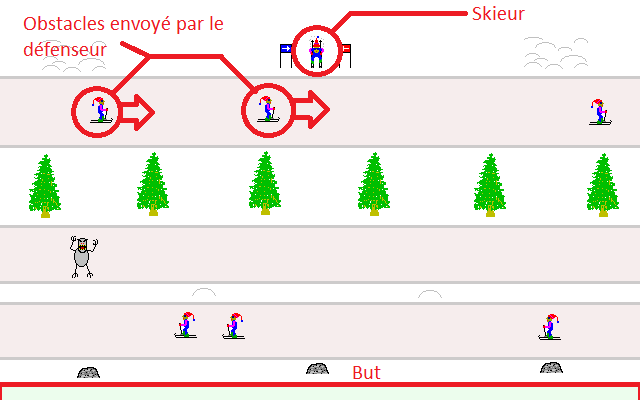
\includegraphics[scale=0.7]{../Screenshots/demo_annotation.png}}
		\caption{Maquette d'une partie}
		\label{fig:maquette}
	\end{figure}
	
	Les zones rouges sont les zones à disposition du joueur 2 pour placer les obstacles, les sapins sont des obstacles fixes. Le joueur 1 gagne s'il atteint la zone en vert sans heurter d'obstacle.
	
	
	\subsection{Utilisation de l'applicatif}
	Le joueur 1 contrôle son personnage à l'aide des flèches du clavier ($\leftarrow$: à gauche, $\downarrow $: en bas, $\rightarrow$: à droite) et tente d'éviter les obstacles. Le joueur 2 place les obstacles dans les colonnes, ceci fait que l'obstacle se met en mouvement dans la colonne. Une bouteille de Fendant\texttrademark se vide au fur et à mesure que le joueur 2 place des obstacles. Il doit ensuite attendre qu'elle se remplisse à nouveau pour placer de nouveaux obstacles.\par
	
	L'administrateur peut régler les paramètres du jeu (« skin » du jeu, vitesse des obstacles, vitesse de rechargement de la bouteille de Fendant\texttrademark). L'administrateur est un rôle hérité de celui de joueur (un administrateur est donc avant tout un joueur). Ce droit est stocké dans la base de données.
	
	
	\subsection{Règles du jeu}
	Pour le joueur 1: le but est d'arriver en bas de la piste sans avoir heurté d'obstacle. \\
	Pour le joueur 2: le but est que le joueur 1 heurte un obstacle.
	
	
	\subsection{Contraintes}
	Le joueur 1 ne peut pas revenir en arrière, une fois descendu une portion de piste il peut s'arrêter, changer de «colonne» ou de continuer à descendre. \par
	
	Le joueur 2 peut envoyer des obstacles pour autant que la bouteille de Fendant\texttrademark ne soit pas vide.
	
	
	\subsection{Priorités de développement}
	\begin{enumerate}
		\item Première version du jeu «standalone» avec un seul joueur qui prend le rôle du joueur 1 (descendre la piste). Les obstacles sont envoyés aléatoirement. (En parallèle, développement du serveur et de l'API).
		\item Ajout du deuxième joueur en local (les deux jouent sur la même machine avec des touches différentes du clavier).
		\item Les joueurs jouent chacun sur leur machine et se connectent à un serveur distant centralisant la partie. Lorsqu'un joueur se connecte, il voit la liste des parties créées (soit en attente d'un joueur, soit en cours). Il peut soit rejoindre une partie en attente d'un joueur soit créer une nouvelle partie.
		\item L'administrateur peut configurer le serveur (paramètres des parties).
	\end{enumerate}
	
	
	\subsection{Base de données}
	La base de données stocke et partage les informations suivantes entre les joueurs et l'administrateur :
	\begin{itemize}
		\item Informations des joueurs (nom d'utilisateur, mot de passe, rôle, points totaux gagnés)
		\item Informations des parties (joueurs, points remportés par chacun)
		\item Paramètres de l'application (ce qui peut être configuré par l'administrateur)
		\item Logs de l'application
	\end{itemize}
	
	
	%
	% ANALYSE
	%
	\section{Analyse}
	
	
	\subsection{Partage des responsabilités entre le serveur et le client}
	
	\subsubsection{Responsabilités du client}
	Le client est en charge de transmettre les actions effectuées par le joueur au serveur. Ces actions sont en fait les touches appuyées qui correspondent à  une action spécifique dans le jeu (comme par exemple aller à droite ou à gauche, ou envoyer un obstacle à un endroit spécifique). Le client doit aussi gérer l'affichage du jeu, en récupérant les emplacements de tous les éléments du jeu (skieur, obstacles fixes et obstacles dynamiques) à partir du serveur.
	
	\subsubsection{Responsabilités du serveur}
	Le serveur lui doit gérer la logique du jeu. Pour chaque action effectuée par un des joueurs, il va mettre à jour les emplacements des éléments du jeu et vérifie si la partie est gagnée (ou perdue) en regardant s'il y a eu une collision ou si le skieur est arrivé en bas de la piste de ski. Il fait ces mises à jour de manière asynchrone, mais il va contacter les clients de manières synchrones (toutes les x millisecondes) pour que les deux joueurs aient le jeu dans le même état chacun.
	
	\subsection{Diagramme d'activité général}
	La figure~\ref{fig:diagramme_activite} représente le diagramme d'activité qui illustre la répartition des responsabilités entre le client et le serveur.
	\begin{figure}[!ht]
		\centering
		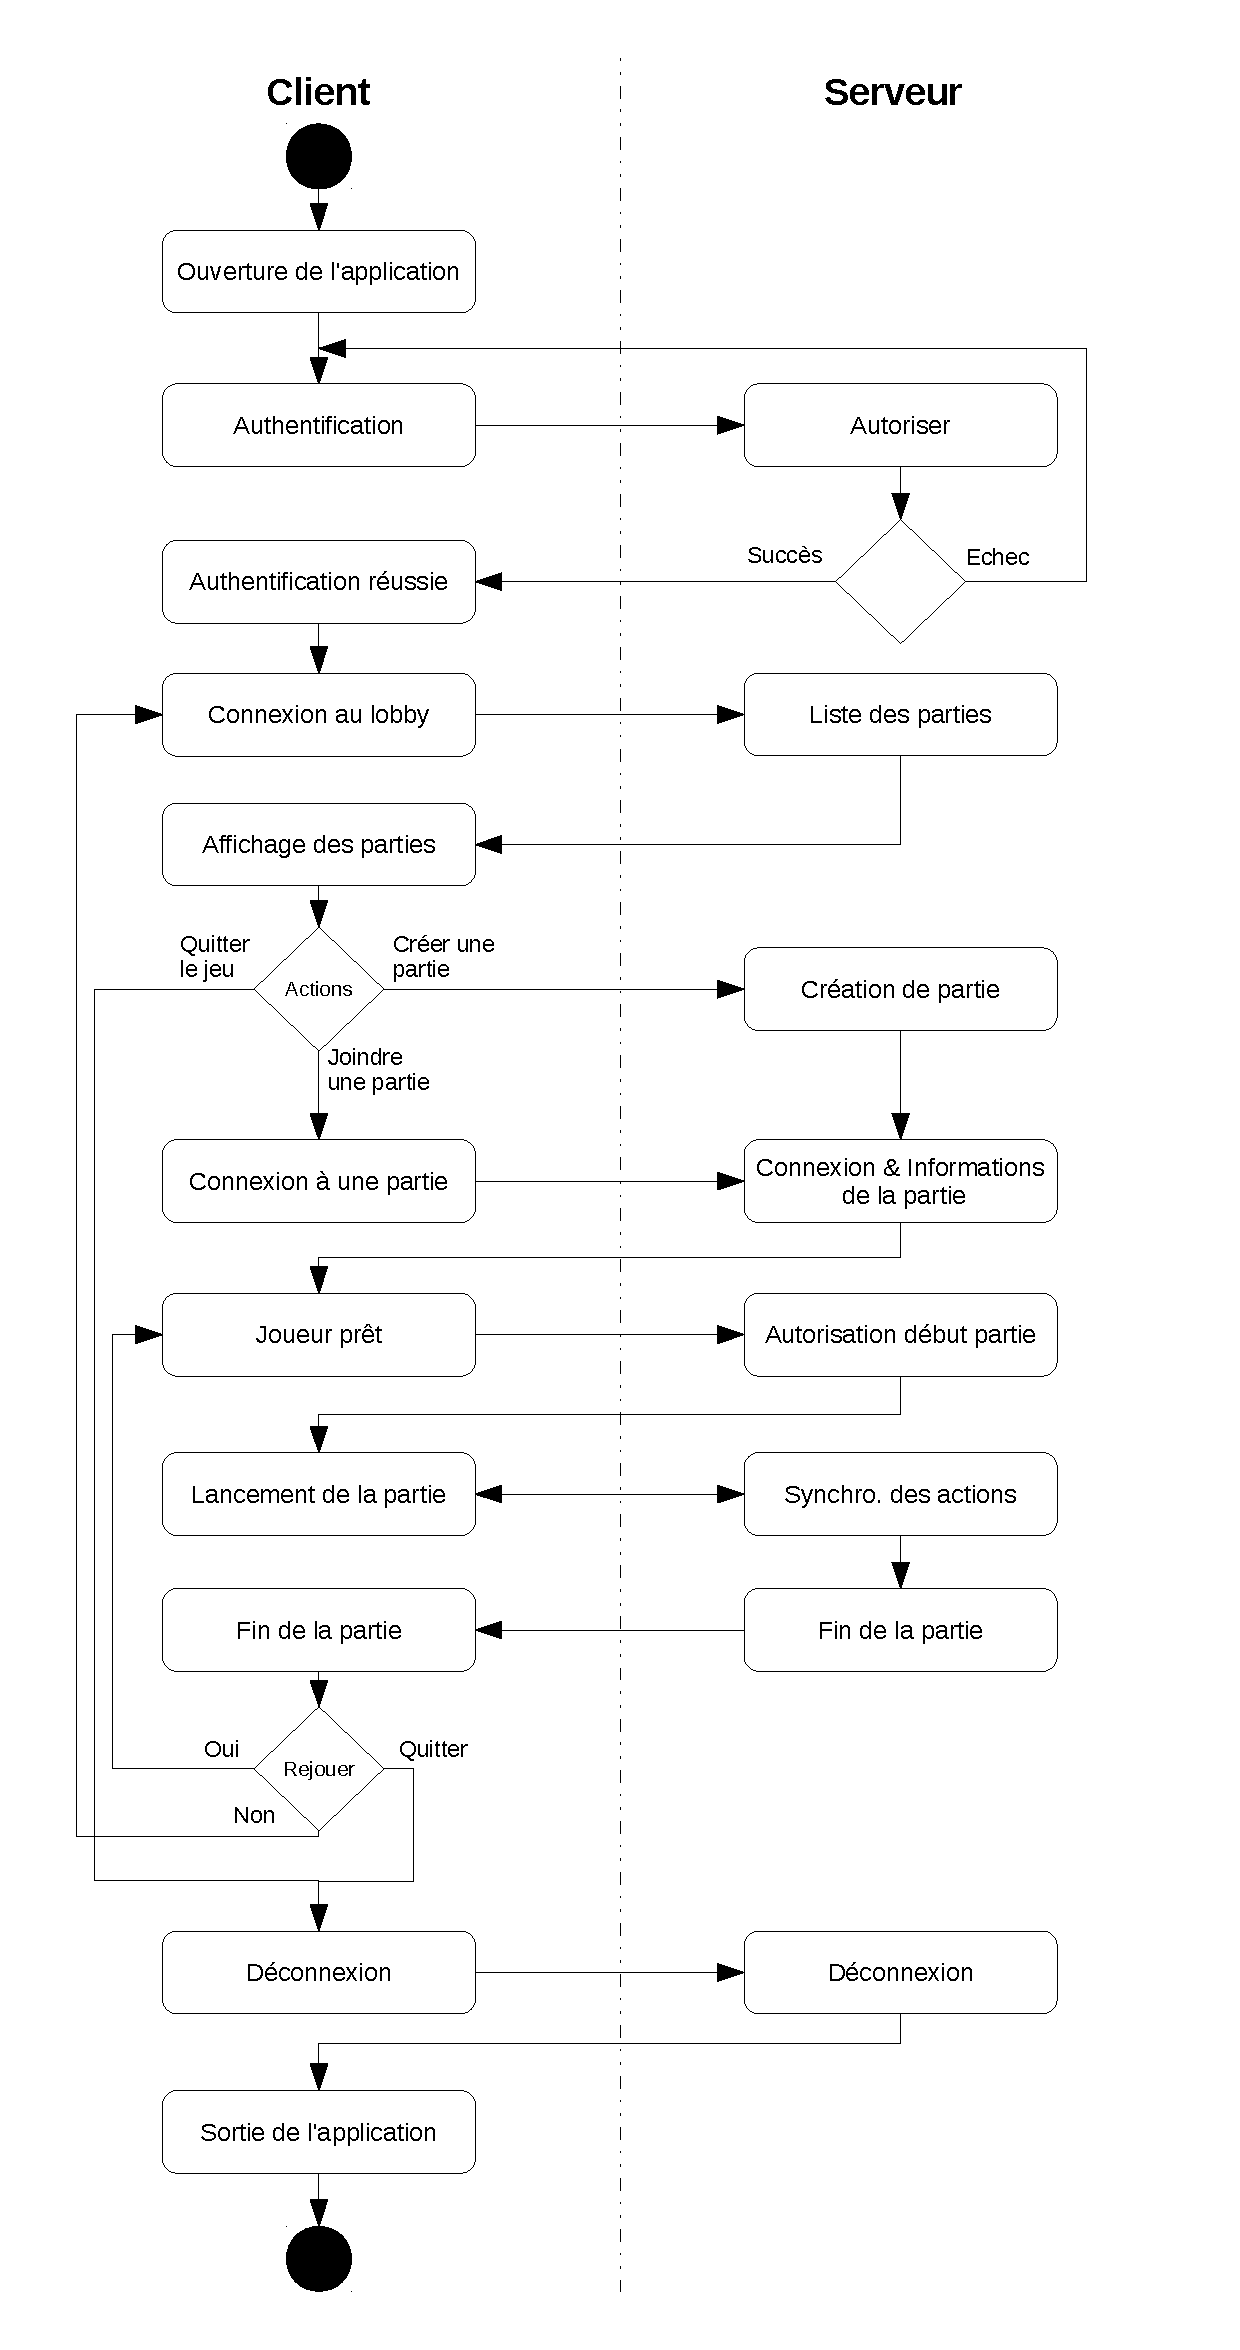
\includegraphics[scale=0.6]{Diagramme_Activite.pdf}
		\caption{Diagramme d'activité}
		\label{fig:diagramme_activite}
	\end{figure}
	
	
	\subsection{Rôle des participants}
	\textbf{Joueurs} : 2 personnes par partie, le \textit{skieur} ayant pour but de réussir à descendre la piste, tandis que l'autre essaye de l'en empêcher (\textit{défenseur}). \\
	
	\textbf{Administrateur} : Peut changer les règles générales du jeu (configuration des difficultés, tailles des cartes, etc...), et s'occuper des données (nettoyer, modifier des joueurs, etc...)
	
	
	\subsection{Cas d'utilisation}
	
	\subsubsection{Diagramme général de contexte}
	\begin{figure}[!ht]
		\centering
		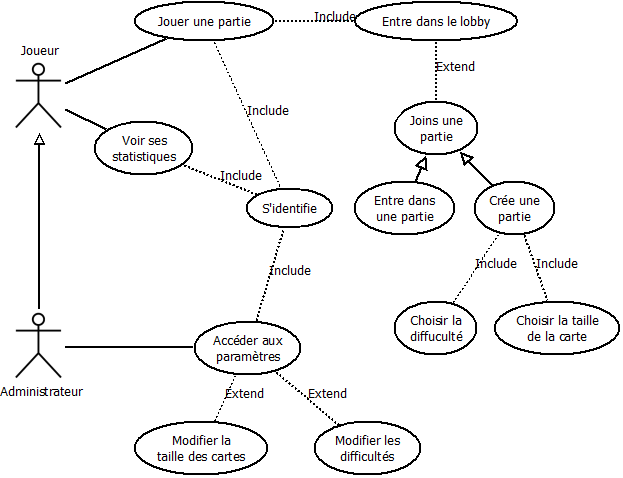
\includegraphics[scale=0.6]{diagramme_utilisation.png}
		\caption{Diagramme d'utilisation}
		\label{fig:diagramme_utilisation}
	\end{figure}
	
	\subsubsection{Description des acteurs}
	\begin{enumerate}
		\item Joueurs, dans une partie nommée : \textit{Skieur} et \textit{Défenseur}
		\item Administrateur
	\end{enumerate}
	
	\subsubsection{Scénario principal}
	\begin{enumerate}
		\item L'un des deux joueurs se connecte au lobby et crée une partie en spécifiant les paramètres qu'il souhaite.
		\begin{enumerate}
			\item Difficulté
			\item Taille de la carte
			\item Son rôle (\textit{Skieur} ou \textit{Défenseur})
		\end{enumerate}
		\item Le second joueur rejoint la partie libre du joueur 1 dans le lobby et prend le rôle restant.
		\item Lorsque les 2 joueurs sont prêts, la partie commence.
		\begin{enumerate}
			\item "\textit{Le skieur}" tente de traverser la piste en déplaçant son personnage de haut en bas.
			\item "\textit{Le défenseur}" tente de l'en empêcher en envoyant des obstacles de gauche à droite.
			\item La partie se termine si le skieur n'a plus de vie ou si il a atteint l'autre côté (le but).
		\end{enumerate}
		\item À la fin de la partie, soit les rôles s'inversent et on recommence une partie à l'étape 3, soit les joueurs quittent la partie. Cette dernière est donc interrompue et les joueurs retournent au lobby.
	\end{enumerate}
	
	\subsubsection{Extensions (ou scénarios alternatifs)}
	Pour permettre la récupération des parties de manière correcte, il faut s'assurer que tous les états et les événements sensibles du système peuvent être récupérés à n'importe quelle étape du scénario. \\
	
	Lors d'une partie, si l'un des deux joueurs est déconnecté, l'adversaire gagne automatiquement la partie et est renvoyé au lobby.
	
	\subsubsection{Scénario d'administration}
	\begin{enumerate}
		\item l'administrateur se connecte à l'interface.
		\item Il modifie l'une des options à sa disposition :
		\begin{enumerate}
			\item Les paramètres du jeu.
			\item Les données d'un joueur.
		\end{enumerate}
		\item puis il peut se déconnecte ou recommencer à l'étape 2.
	\end{enumerate}
	
	
	\subsection{Modèle de domaine}
	La figure~\ref{fig:model_domain} représente une ébauche du modèle de domaine.
	
	\begin{figure}[!ht]
		\centering
		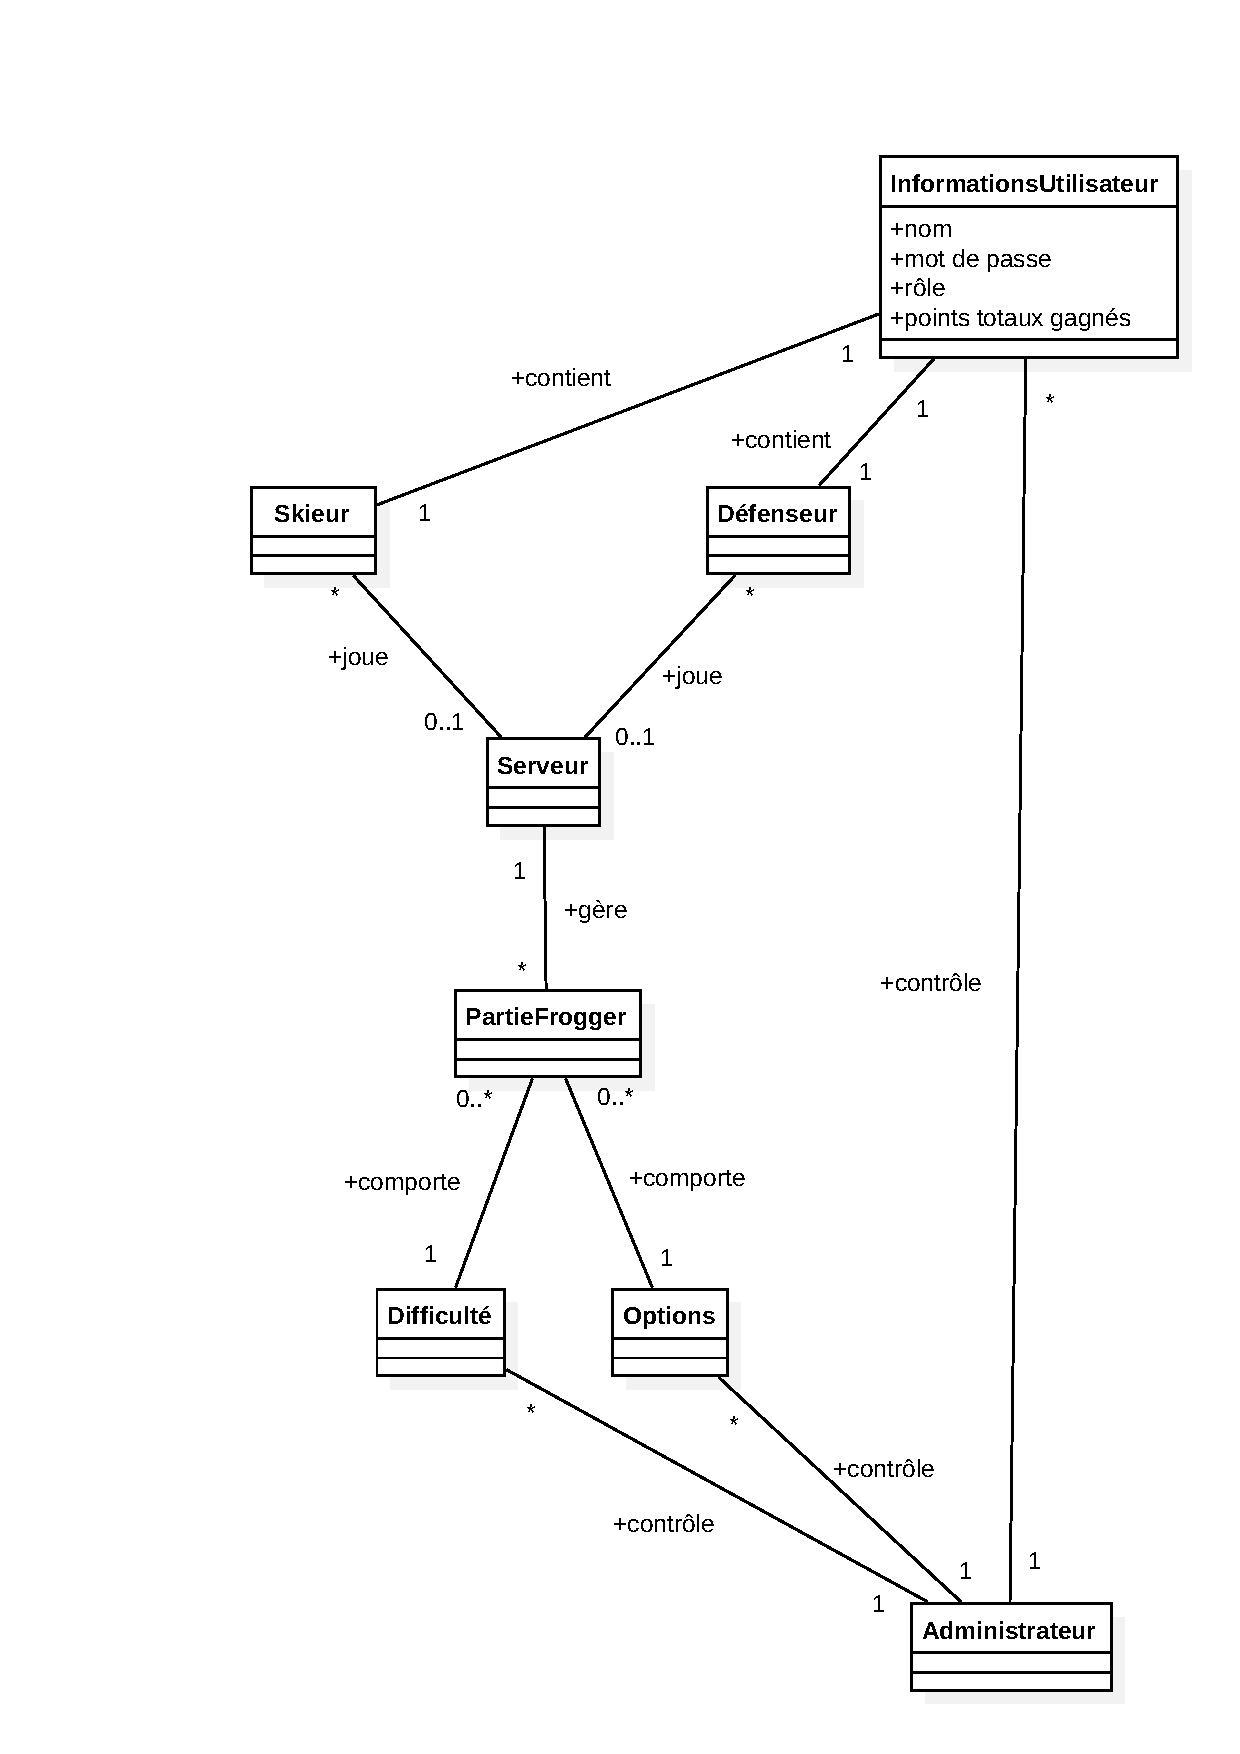
\includegraphics[scale=0.6]{../Schemas/model_domain.pdf}
		\caption{Modèle de domaine}
		\label{fig:model_domain}
	\end{figure}
	
	\subsubsection{Modèle de domaine pour le client}
	\subsubsection{Modèle de domaine pour le serveur}
	
	
	\subsection{Base de données}
	L'objectif de la base de données est principalement de stocker les paramètres du jeu et les données utilisateurs. Nous avons fait le choix de ne pas stocker d'informations concernant les parties en cours qui seront chargées uniquement dans la mémoire du serveur. \par
	
	On trouve donc une entité \texttt{User} qui peut être \texttt{Administrator}, dont on stocke le login et le nombre de victoires. \texttt{Settings} modélise les réglages généraux du jeu, \texttt{MapSize} permettra à l'utilisateur qui crée une partie de choisir parmi plusieurs tailles de carte. \texttt{DifficultyLevel} modélise les niveaux de difficulté parmi lesquels l'utilisateur créant la partie aura le choix.
	
	\begin{figure}[ht]
		\centering
		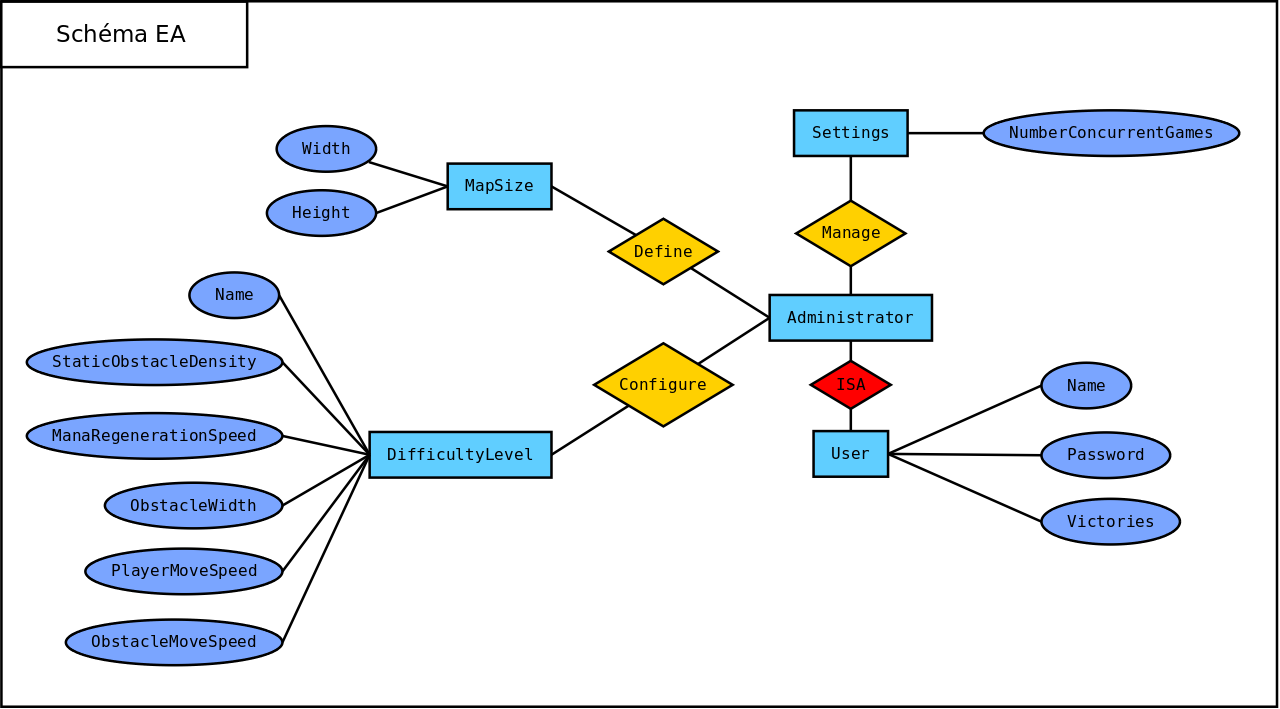
\includegraphics[width=\textwidth]{../Database/ER_diagram.png}
		\caption{Modèle conceptuel}
		\label{fig:database_er}
	\end{figure}
	
	\subsubsection{Modèle conceptuel (entité-associations)}
	
	
	%
	% CONCEPTION DU PROJET
	%
	\section{Conception du projet}
	
	
	\subsection{Protocole d'échange entre le client et le serveur}
	\subsubsection{Communication}
	Nous allons utiliser JSON\footnote{JSON : JavaScript Object Notation} comme protocole d'échange entre le client et le serveur. \par
	En effet, de par la structure de son contenu, l'échange d'information entre les deux intervenants est très facilement sérialisable/désérialisable, sans compter sur le fait que le contenu est lisible par un individu (contrairement à un contenu binaire).
	
	\subsubsection{Données échangées}
	L'API de communication en cours d'élaboration se trouve sur le wiki de notre projet GitHub \\ \url{https://github.com/gluthier/GEN-projet/wiki/Communication-API} \\
	L'idée est que chaque joueur envoie au serveur ses commandes : pour le skieur s'il souhaite tourner à gauche ou à droite, pour le Valaisan sur quelle ligne il envoie un obstacle. Le serveur s'occupe de placer les obstacles et le skieur et envoie les positions de manière régulière aux deux clients. Les clients ne font que l'affichage et l'envoi de commande alors que le serveur s'occupe de la synchronisation, gestion des collisions, etc.
	
	
	\subsection{Diagrammes de classes du serveur et du client}
	
	\subsection{Modèle conceptuel \& relationnel de la base de données}
	
	
	%
	% IMPLEMENTATION DU PROJET
	%
	\section{Implémentation du projet}
	
	
	\subsection{Structure du projet}
	Pour partager les différentes parties de l'applicatif, nous avons séparé le code en plusieurs projets afin d'exposer que le code qui est nécessaire. Le client, par exemple, n'a pas besoin d'avoir accès au code qui gère la base de données ni à code de l'applicatif administrateur.
	
	\subsubsection{GEN-protocol}
	\texttt{GEN-protocol} définit le protocole utilisé par le client et le serveur pour communiquer entre eux.
	\subsubsection{GEN-BDD}
	\texttt{GEN-BDD} offre une interface pour communiquer avec la base de données du jeu.
	\subsubsection{GEN-server}
	\texttt{GEN-server} est la partie que gère la logique du jeu et la synchronisation des joueurs entre eux.
	\subsubsection{GEN-admin}
	\texttt{GEN-admin} est l'applicatif administrateur qui permet de gérer la base de données, ajouter des comptes utilisateurs, consulter les logs en offrant une interface graphique.
	\subsubsection{GEN-Frogger}
	\texttt{GEN-Frogger} est le code destiné au client qui gère l'affichage graphique du jeu, ainsi que les interactions du joueur.
	
	
	\subsection{Technologies, langages, bibliothèques utilisées}
	Ce projet a été réalisé entièrement en Java, que ce soit le client ou le serveur.
	Nous avons utilisé JavaFX pour gérer la partie graphique du jeu. Il s'agit d'une bibliothèque de création d'interfaces graphiques pour le langage Java. Elle contient notamment des outils pour du graphisme 2D que nous avons utilisés pour la gestion des éléments affichés à l'écran. \\
	
	La bibliothèque \href{https://github.com/TestFX/TestFX}{TestFX} a été utilisée pour mettre en place des tests qui fonctionnent avec JavaFX, car celui-ci demande a besoin que l'application s'exécute réellement pour fonctionner correctement. Les tests unitaires classiques (comme JUnit) ne peuvent pas être utilisés pour tester les parties gérées par JavaFX.
	
	
	\subsection{Technologies "originales" (autres que les technologies étudiées à l'école)}
	
	\subsubsection{Guava}
	\begin{enumerate}
		\item Descriptif
		\href{https://github.com/google/guava}{Guava} est une ensemble de bibliothèque open source développé par Google en Java. Nous l'utilisons principalement pour ses outils de hachage et sur les immutable.
		\item Avantages
		Elles offrent pas mal d'outils au niveau des objets immutable, comme par exemple des table d'association immutable que nous utilisons, et des fonctionnalité au niveau du hachage
		\item Limitations
		La librairie est lourde ce qui peut alourdir notablement le projet.
		\item Remarques personnelles
		Très pratique et simple d'utilisations. Comme elle est utilisée par pas mal de monde, on n'a pas de problème à trouver des solutions aux éventuels problèmes que l'on pourrait rencontré avec.
	\end{enumerate}
	
	\subsection{Problèmes éventuels rencontrés et solutions apportées}
	
	\subsubsection{Logique FX }
	Venant de \textit{Swing}, nous avons eu pas mal de problèmes avec l'utilisation de \textit{JavaFx} et des nouvelles logiques de conception que ça amener. Nous les avons peu à peu résolu, en reprenant bien ce que nous avions fait et en apprenant tout depuis le début.
	
	\subsubsection{ReadLine et \textit{\textbackslash n}}
	Dans notre protocole d'échange nous utilisons du \textit{json} pour communiquer les différents messages nécessaires au bon fonctionnement du jeu, afin de lire les messages nous utilisons la méthode \textit{readLine} qui est bloquante et permet d'attendre sur une notification.
	Cependant nous avons remarqué que pour utiliser readLine, il fallait que nos messages soient bien terminé (via un \textit{\textbackslash n}), pour que la commande nous retourne le message reçu et le traite.
	Nous avons donc ajouter à la fin des paquets \textit{json} un \textit{\textbackslash n} pour nous assurer que cela fonctionnait bien.
	\subsubsection{Partage de classes/code entre plusieurs projets }
	Notre structure étant composé de 4 projets distincts, nous avions besoin de pouvoir partagé des fonctions entre eux de manière simple, et surtout sans copié-collé. 
	Pour palier à ça, nous utilisons le système de gestion \textit{maven}, ce qui nous permet de lié les projets entre eux, d'assurer une dépendance toujours à jour et de facilement construire nos projets.
	
	
	%
	% GESTION DU PROJET
	%
	\section{Gestion du projet}
	
	
	\subsection{Rôle des participants au sein du groupe de développement}
	\begin{enumerate}
		\item Tony Clavien: Analyste, design manager, programmeur, représentant valaisan, responsable apéro
		\item Maxime Guillod: Chef de projet, programmeur
		\item Gabriel Luthier: Responsable des tests, programmeur
		\item Guillaume Milani: Architecte, concepteur en chef, programmeur, community manager
	\end{enumerate}
	
	\subsection{Plan d'itérations initial}
	
	\subsubsection{Création de l'interface de base}
	\begin{enumerate}[labelwidth=5em,leftmargin=8em]
		\objectif Mise en place de l'interface utilisateur de l'écran principal du jeu.
		\duree 1 semaine
		\dateRendu 26.04.2017
		\partageTache Création des images/sprites, affichage de l'UI, mise en place des obstacles fixes
		\effort 15 heures
	\end{enumerate}
	
	\subsubsection{Ajout du 1er joueur avec les obstacles}
	\begin{enumerate}[labelwidth=5em,leftmargin=8em]
		\objectif Développement de la logique du joueur "skieur" qui descend la piste.
		\duree 1 semaine
		\dateRendu 03.05.2017
		\partageTache interaction avec les touches du clavier, déplacement du skieur sur la carte
		\effort 20 heures
	\end{enumerate}
	
	\subsubsection{Ajout du 2ème joueur en local}
	\begin{enumerate}[labelwidth=5em,leftmargin=8em]
		\objectif Développement de la logique du joueur "défendant" qui envoie des obstacles contre l'autre joueur.
		\duree 1 semaine
		\dateRendu 10.05.2017
		\partageTache interaction avec les touches du clavier, logique de déplacement des obstacles sur la carte
		\effort 20 heures
	\end{enumerate}
	
	\subsubsection{Mise en place des logiques de jeu}
	\begin{enumerate}[labelwidth=5em,leftmargin=8em]
		\objectif Détection des collisions entre les obstacles (fixes et mobiles) avec le joueur "skieur", des conditions de victoire et défaite et barre de recharge pour la pose d'obstacles.
		\duree 1 semaine
		\dateRendu 17.05.2017
		\partageTache détection de collisions, conditions de victoire, conditions de défaite, barre de recharge pour la pose d'obstacles
		\effort 20 heures
	\end{enumerate}
	
	\subsubsection{Ajout de la communication avec le serveur}
	\begin{enumerate}[labelwidth=5em,leftmargin=8em]
		\objectif Développement du serveur pour pouvoir jouer à distance.
		\duree 1 semaine
		\dateRendu 24.05.2017
		\partageTache connexion des deux joueurs à une partie, communication réseau entre le serveur et les deux joueurs, gestion de l'état d'une partie
		\effort 30 heures
	\end{enumerate}
	
	\subsubsection{Application administrateur}
	\begin{enumerate}[labelwidth=5em,leftmargin=8em]
		\objectif Développement de l'application administrateur utilisée afin de modifier les paramètres des différents modes de jeu et des données des joueurs.
		\duree 1 semaine
		\dateRendu 31.05.2017
		\partageTache UI de l'applicatif, connexion à la base de données, fonctions de modification de la BD
		\effort 20 heures
	\end{enumerate}
	
	\subsubsection{Ajout du Lobby}
	\begin{enumerate}[labelwidth=5em,leftmargin=8em]
		\objectif Gestion du lobby (UI et logique).
		\duree 1 semaine
		\dateRendu 07.06.2017
		\partageTache UI du lobby (menu), récupérer les informations sur les parties en recherche de joueurs, création d'une nouvelle partie
		\effort 20 heures
	\end{enumerate}
	
	\subsubsection{Finalisation}
	\begin{enumerate}[labelwidth=5em,leftmargin=8em]
		\objectif Finalisation de l'application et ajout de bonus.
		\duree 1 semaine
		\dateRendu 14.07.2017
		\partageTache derniers détails, mise en places des bonus/easter eggs
		\effort 15 heures
	\end{enumerate}
	
	
	\subsection{Suivi du projet}
	
	\subsubsection{Itération 1: Création de l'interface de base}
	Cette itération a été consacrée à la découverte de la bibliothèque JavaFX pour afficher l'interface de base. L'image du fond et les différents sprites du jeu ont été mis en place, ainsi que la grille où tous les éléments seront affichés. Pas de problèmes ont été rencontrés et donc aucune replanification n'est nécessaire.
	
	\subsubsection{Itération 2: Ajout du 1er joueur avec les obstacles}
	Le premier joueur (le skieur) est mis en place et peut se déplacer à travers la grille (pas case par case, cela sera développé plus tard). Le premier problème rencontré a été d'écrire des tests qui fonctionnent avec JavaFX. En effet, des tests unitaires (JUnit) classiques ne fonctionnent pas, car JavaFX a besoin que le jeu s'afficher "en vrai" pour pouvoir s'exécuter correctement (par exemple pour répondre à un clique du joueur, il a besoin de savoir à quelle position il a cliqué pour éventuellement interagir avec l'élément cliqué). Aucune replanification a été faite, les tests seront simplement développés ensuite au fil des itérations.
	
	\subsubsection{Itération 3: Ajout du 2ème joueur en local}
	La création des obstacles dynamiques qui sont créés par le 2ème joueur (à l'aide de son clavier) a été mise en place. Les collisions avec le skier ont aussi été développée, mais le code n'a pas encore été mergé à ce moment-là et les deux fonctionnalités marchent, mais séparément. La bibliothèque \href{https://github.com/TestFX/TestFX}{TestFX} a été choisie et testée pour effectuer nos tests fonctionnant avec JavaFX. Pas de replanification a été faite, mais le bug des collisions devra être corrigé par la suite.
	
	\subsubsection{Itération 4: Mise en place des logiques de jeu}
	Remise en question générale et changement du déplacement du skieur pour rendre la détection des collisions plus facile et aussi par anticipation à la mise en place du serveur. En effet, comme c'est lui qui devra gérer la logique du jeu, on diminue ainsi le nombre de requêtes qui lui seront transmises. Une grosse partie de travail effectué lors de cette itération à été de changer le fonctionnement interne du jeu, l'ajout de nouvelles fonctionnalités en a donc péri.
	
	Cette fois-ci, une replanification est nécessaire. Les trois cas d'utilisation qui auraient dû être développés se voient partagés dans les itérations suivantes. L'UC \textit{Jouer une partie} et l'UC \textit{S'identifie} sont reporté à l'itération 5 tandis que l'UC \textit{Voir ses statistiques} se reportent à l'itération 6.
	
	\subsubsection{Itération 5: Ajout de la communication avec le serveur}
	Cette itération nous a pris beaucoup plus de temps que prévu. On a décidé de se concentrer sur le case d'utilisation \textit{Jouer une partie}, qui constitue le cœur du jeu. Il a été possible de finaliser ce case d'utilisation, mais cela nous a demandé de refactorer presque l'ensemble du projet pour implémenter les collisions entre les obstacles, la logique de victoire/défaite d'une partie et l'interface pour pouvoir relancer une partie.
	
	L'UC \textit{S'identifie} a quand même été entamée. La base de données qui contiendra les informations des utilisateurs, les logs ainsi que les paramètres du jeux a été mise en place. Il reste cependant à faire communiquer le client avec le serveur pour effectivement pouvoir s'identifier.
	
	Pour pouvoir finir ce cas d'utilisation, on effectue une replanification et déplace l'UC \textit{S'identifie} à l'itération suivante (la 6).
	
	\subsubsection{Itération 6: Application administrateur}
	L'application de l'interface d'administration est développée avec une interface sommaire pour le moment. Un affichage des logs du serveur avec un système d'ID pour le suivi de chaque instance (de chaque joueur qui se connecte au serveur) est implémenté. L'interface du login est aussi mise en place, mais la communication avec le serveur n’est toujours pas fonctionnelle. Un gros travail sur les divers éléments de communication est fourni, mais rien n'est encore fonctionnel à 100\%.
	
	Une replanification est faite pour reporter tous les cas d'utilisation qui nécessitent de communiquer avec le serveur à l'itération suivante.
	
	\subsubsection{Itération 7: Ajout du Lobby}
	Les paramètres des jeux sont maintenant configurables dans un onglet dans l'interface administrateur. Tous ces paramètres sont fonctionnels, enregistrés dans la base de données et communiqués par la suite au client par le serveur. Le principal du travail a été fourni sur le backend, il n'y a donc pas grand-chose de nouveau à montrer. Le problème principal est que tout a été très bien avancé, mais rien à 100\%. On a donc pour l'instant une application qui n'est pas fonctionnelle.
	
	La replanification est plutôt simple: on reporte tout pour la dernière itération.
	
	\subsubsection{Itération 8: Finalisation}
	Pour cette itération, on a du travailler sur tout le projet en général, car il a fallut terminer de développer le maximum de fonctionnalité qu'il nous manquait et surtout corriger les bugs pour rendre l'application fonctionnelle. 
	
	
	\subsection{Stratégie de tests}
	Nous avons effectué quelques tests pour les parties importantes de l'application. Généralement, la personne qui développait une fonctionnalité faisait elle-même les tests nécessaires pour assurer le bon fonctionnement du programme. Tout n'a pas été testé, car on a été rattrapé par les deadlines. 
	
	Pour faire ces tests, on a utilisé un mélange de JUnit pour tout ce qui est une application Java uniquement et TestFX pour les parties utilisant JavaFX (il s'agit de la partie client du jeu).
	
	\subsubsection{Utilisation de JUnit pour une classe définissant le protocole}
	\lstinputlisting{../Application/protocol/protocol/src/test/java/ch/heigvd/protocol/ProtocolTest.java}
	
	\subsubsection{Résultats des tests}
	La figure~\ref{fig:resTests} montre le résultat des tests JUnit.
	\begin{figure}[ht]
		\centering
		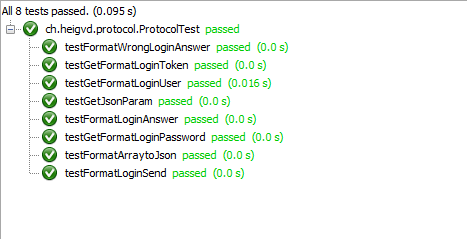
\includegraphics{tests.png}
		\caption{Résultats des tests JUnit}
		\label{fig:resTests}
	\end{figure}
	
	
	\subsection{Stratégie d'intégration du code de chaque participant}
	Afin de collaborer efficacement, nous avons utilisé Git (avec la plateforme Github) pour gérer l'intégration du code de chaque développeur. Pour chaque fonctionnalité, une branche était créée pour permettre à différentes personnes de collaborer dessus. Puis, quand la fonctionnalité était finie, une pull request était ouverte sur Github pour permettre aux autres membres du groupe d'analyser et critiquer (si besoin) les changements effectués. Une fois tout le monde satisfait, la pull request était mergée sur la branche master qui correspond à l'ensemble de fonctionnalités finies.
	
	%
	% ETAT DES LIEUX
	%
	\section{État des lieux}
	
	
	\subsection{Ce qui fonctionne (résultats des tests)}
	
	
	\subsection{Ce qu'il resterait à développer (en proposant une planification)}
	
	
	%
	% AUTO-CRITIQUE
	%
	\section{Auto-critique}
	
	Notre principale difficulté a été de commencer à développer l'application en local puis ensuite de vouloir la transformer pour pouvoir jouer à travers un serveur. Beaucoup d'effort a été fourni pour la rendre fonctionnelle à deux joueurs sur un ordinateur et il a fallu presque tout refaire la logique du jeu pour pouvoir communiquer avec le serveur.
	
	Un autre aspect qu'on aurait pu mieux faire a été notre dispersion. Au fil des itérations et surtout des replanifications, la charge de travail c'est accumulée et on avait de plus en plus de fonctionnalités à développer. Au lieu de se focaliser sur l'essentiel, on a profité d'être 4 et à chaque fois on a partagé le travail dans l'espoir de tout finir. On a donc pas pu développer toutes les fonctionnalités que l'on avait prévu lors de la planification du projet.
	
	On a aussi eu plus de peine à gérer la fin de semestre et tous les rendus des autres cours qui viennent en même temps. Pour améliorer ça, on aurait pu, lors des replanifications, oser redéfinir les fonctionnalités pour enlever celles qui ne sont pas essentielles (notamment les statistiques ou le lobby par exemple) pour pouvoir se concentrer sur l'aboutissement du cœur du jeu.
	
	
	%
	% CONCLUSION
	%
	\section{Conclusion}
	Pour conclure, ce projet aura été une belle expérience. En effet, on a beaucoup appris des difficultés qui peuvent survenir lorsque l'on entreprend de développer un projet de plus grande envergure que ce à quoi on a été habitué de développer de notre côté. Une des leçons a été l'importance d'une bonne planification et replanification si besoin. On a plutôt eu tendance à simplement repousser le travail des itérations qui n'avait pas été fini aux itérations suivantes sans réfléchir vraiment si c'était une bonne idée.
	
	Malgré l'utilisation d'outils tels que Trello et Github, la collaboration n'a pas été aisée. Planifier les itérations et ensuite partager le travail demande pas mal de temps. Ensuite, plus le projet avance, plus l'on est dépendant du bon développement des collègues. Il nous est arrivé de nous retrouver dans la situation que, malgré l'accès à l'historique des modifications apportées par chacun, de remodifier le changement et ainsi revenir en arrière parce que l'on n’avait pas aperçu la raison du changement plus loin dans le code.
	
	On peut également ajouter que le temps nécessaire à une programmation propre, claire et facilement adaptable par la suite a été négligé. En effet, bon nombre de changements ont du s'effectuer a posteriori de leur développement, ce qui de par la qualité du code des premières itérations, nous à demandé un effort supplémentaire et non prévu. 
	
	Malgré tout, même si l'on n'a pas réussi à terminer entièrement le projet tel que l'on avait planifié en début de semestre, on a pu développer une bonne partie, en prenant soin de bien structurer notre application. On a pu mettre en place une base de données ainsi qu'une API permettant d'y accéder sans devoir écrire toutes les requêtes SQL "à la main". Notre partie administration fonctionne bien aussi. On peut accéder aux logs de tous ce qu'il se passe dans l'application, ce qui est utile non seulement en phase debug, mais aussi lors du cours normal pour pouvoir vérifier que tout fonctionne correctement. Le protocole que l'on a défini est aussi bien abouti. Le fait de l'avoir séparé du client et du serveur nous permet de simplement le définir une seule fois et laisser ensuite et le client et le serveur le soin d'aller chercher les informations qu'ils ont besoin pour communiquer entre eux. Et surtout, on peut effectivement jouer en réseau sur des machines différentes. Le jeu n'est pas extrêmement équilibré, mais au moins il est jouable.
	
	En somme, ce projet nous a beaucoup appris sur le cycle complet (accéléré dans notre cas) d'un développement à partir de la phase d'initialisation jusqu'à la fin de celle de construction, en passant par la phase d'élaboration et en s'arrêtant avant celle de transition qui serait celle où l'on livre l'application finale au client. Ces connaissances sont très utiles pour la suite dans le monde professionnel.
	
	%
	% MAUEL D'UTILISATION
	%
	\appendix
	\section{Manuel d'utilisation} \label{app:manuelUtil}
	
	\subsection{Installation}
	On a plusieurs manières pour jouer. La première, la plus simple, consiste à lancer les fichiers \texttt{.jar} du serveur pour lancer un serveur et de Frogger pour lancer un client.
	
	La deuxième méthode consiste à compiler depuis le code source. Pour cela, il faut compiler séparément les projets suivants: \texttt{GEN-protocol}, \texttt{GEN-BDD}, \texttt{GEN-admin}, \texttt{GEN-server} puis \texttt{GEN-Frogger}. L'ordre est important car certain projets sont des dépendances d'autres.
	
	Ensuite, pour jouer, il faut évidemment qu'un serveur tourne quelque part. L'adresse du serveur peut être configurée dans le code dans \texttt{ch-heigvd.frogger.Client.Constants}. Ensuite lancer au moins deux clients. Le premier doit créer une partie (ou attendre que le deuxième se connecte et crée lui une partie). Ensuite l'autre client se connecte à la partie et ils peuvent enfin se mettre à jouer.
	
	\subsection{Utilisation}
	
	\begin{enumerate}
		\item Pour commencer, il faut d'abord se login dans l'application. La figure~\ref{fig:login} montre cette étape.
		\item Ensuite, on arrive dans le lobby. On a l'option de soit créer une partie, soit en rejoindre une. La figure~\ref{fig:lobby} montre quand le premier joueur se connecte et arrive dans le lobby vide.
		\item La figure~\ref{fig:nouvellePartie} montre l'interface de création d'une nouvelle partie.
		\item Après avoir créé un partie, le joueur arrive dans le jeu et est en attente d'un nouveau joueur pour pouvoir commencer le jeu. La figure~\ref{fig:jeuSkier} montre cette étape.
		\item Quand le deuxième joueur se connecte, la partie peut alors commencer. La figure~\ref{fig:jeu} montre une partie en cours.
	\end{enumerate}	

	\begin{figure}[ht]
		\centering
		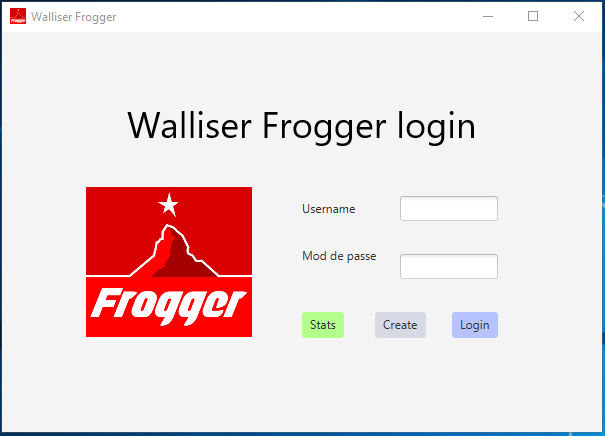
\includegraphics[width=\textwidth]{../Screenshots/login.png}
		\caption{Le login}
		\label{fig:login}
	\end{figure}

	\begin{figure}[ht]
		\centering
		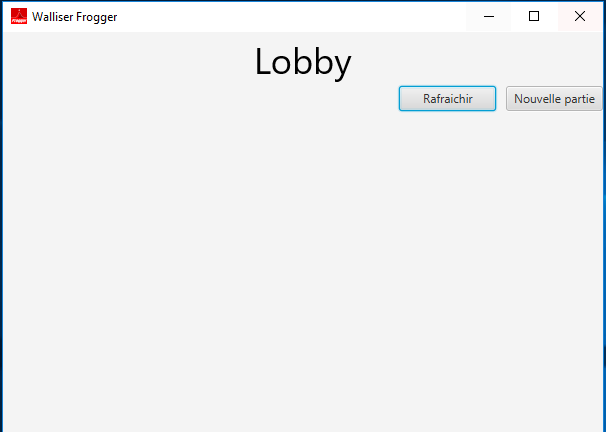
\includegraphics[width=\textwidth]{../Screenshots/lobby.png}
		\caption{Le lobby}
		\label{fig:lobby}
	\end{figure}
	
	\begin{figure}[ht]
		\centering
		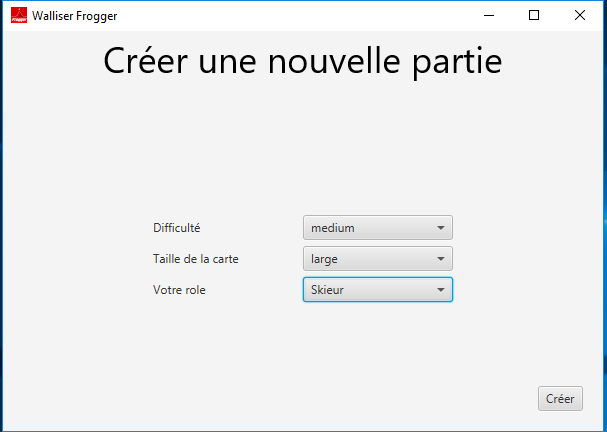
\includegraphics[width=\textwidth]{../Screenshots/nouvelle_partie.png}
		\caption{Création d'une nouvelle partie}
		\label{fig:nouvellePartie}
	\end{figure}
	
	\begin{figure}[ht]
		\centering
		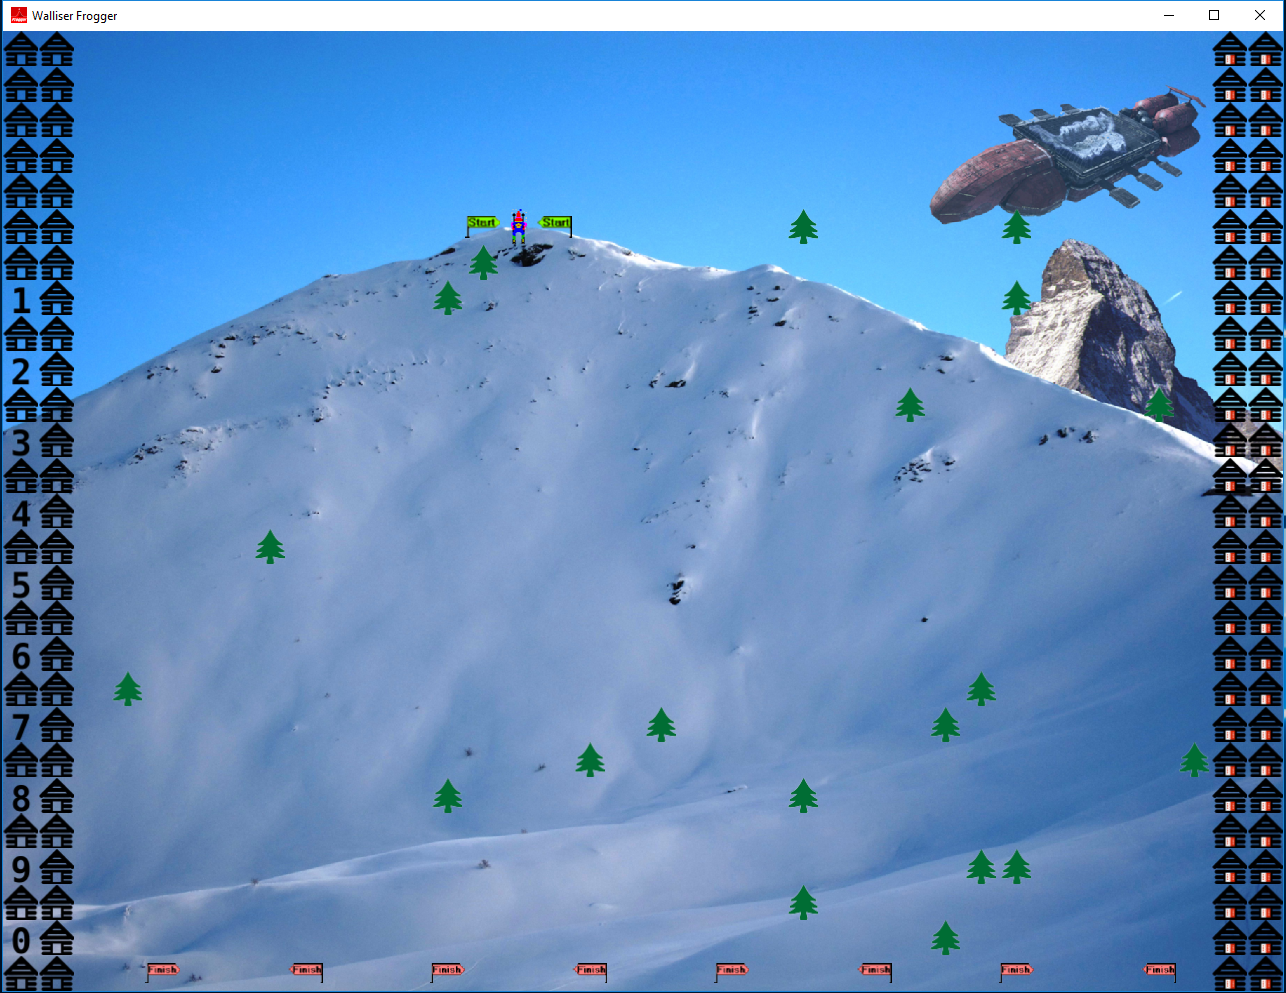
\includegraphics[width=\textwidth]{../Screenshots/jeu_skier.png}
		\caption{Jeu lancé avec seulement le skieur}
		\label{fig:jeuSkier}
	\end{figure}
	
	\begin{figure}[ht]
		\centering
		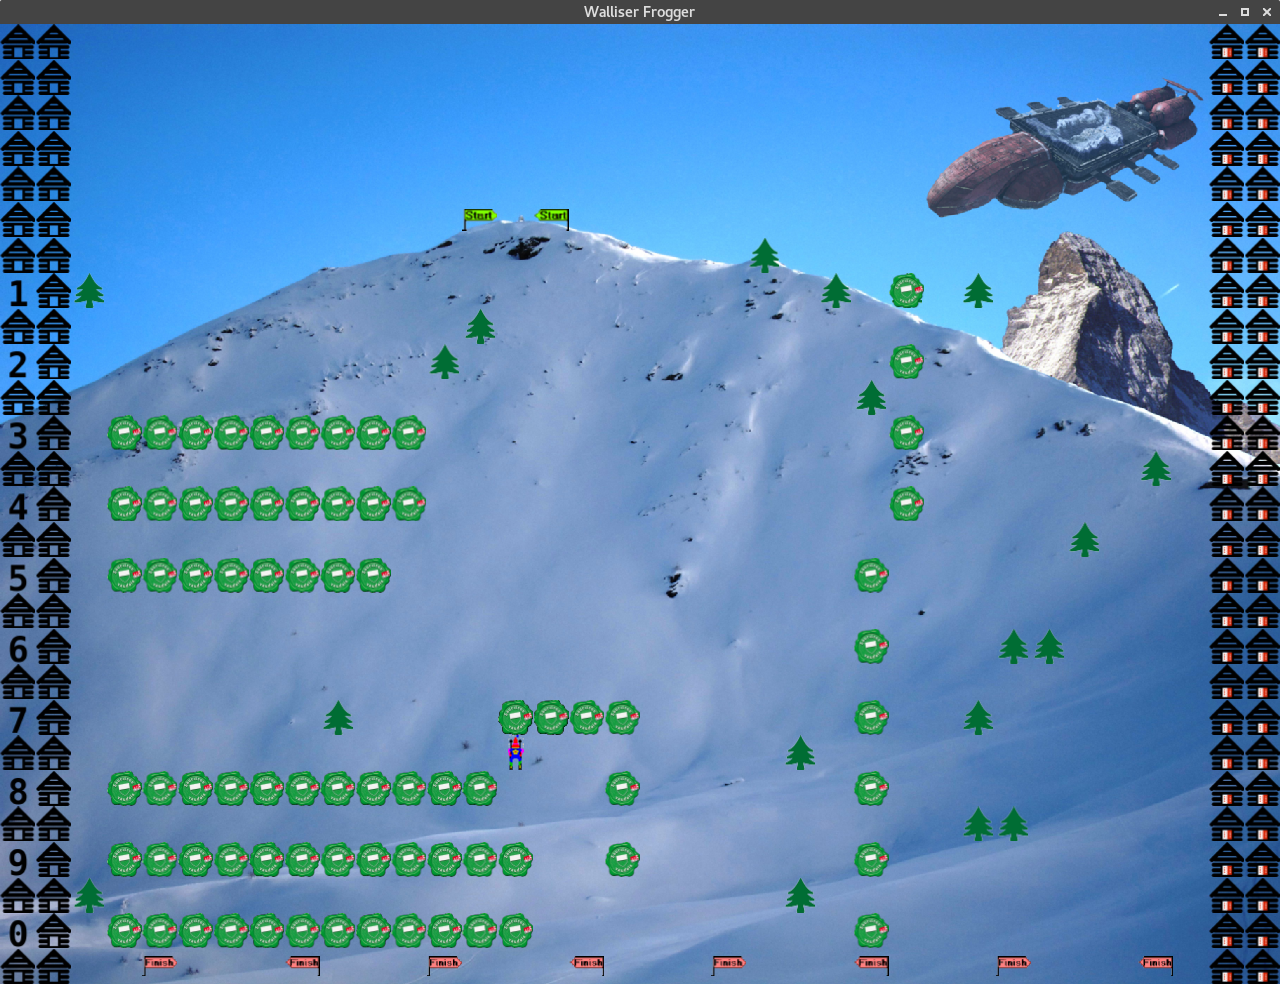
\includegraphics[width=\textwidth]{../Screenshots/jeu.png}
		\caption{Jeu avec 2 clients connecté à une partie}
		\label{fig:jeu}
	\end{figure}
		
	
\end{document}

